\section{\RU{Пример с сравнением}\EN{Comparison example}}

\RU{Попробуем теперь вот это:}\EN{Let's try this:}

\lstinputlisting{patterns/12_FPU/3_comparison/d_max.c}

\RU{Несмотря на кажущуюся простоту этой функции, понять, как она работает, будет чуть сложнее.}
\EN{Despite the simplicity of the function, it will be harder to understand how it works.}

% subsections
\subsection{x86}

% subsubsections
\subsubsection{\NonOptimizing MSVC}

\RU{Вот что выдал MSVC 2010}\EN{MSVC 2010 generates the following}:

\lstinputlisting[caption=\NonOptimizing MSVC 2010]{patterns/12_FPU/3_comparison/x86/MSVC/MSVC.asm.\LANG}

\index{x86!\Instructions!FLD}
\RU{Итак, \FLD загружает \TT{\_b} в регистр \ST{0}.}
\EN{So, \FLD loads \TT{\_b} into \ST{0}.}

\label{Czero_etc}
\newcommand{\Czero}{\TT{C0}\xspace}
\newcommand{\Ctwo}{\TT{C2}\xspace}
\newcommand{\Cthree}{\TT{C3}\xspace}
\newcommand{\CThreeBits}{\Cthree/\Ctwo/\Czero}

\index{x86!\Instructions!FCOMP}
\RU{\FCOMP сравнивает содержимое \ST{0} с тем, что лежит в \TT{\_a} и выставляет биты \CThreeBits в 
регистре статуса FPU. Это 16-битный регистр отражающий текущее состояние FPU.}
\EN{\FCOMP compares the value in \ST{0} with what is in \TT{\_a} 
and sets \CThreeBits bits in FPU 
status word register, accordingly. 
This is a 16-bit register that reflects the current state of the FPU.}

\RU{После этого инструкция \FCOMP также выдергивает одно значение из стека. 
Это отличает её от \FCOM, которая просто сравнивает значения, оставляя стек в таком же состоянии.}
\EN{After the bits are set, the \FCOMP instruction also pops one variable from the stack. 
This is what distinguishes it from \FCOM, which is just compares values, leaving the stack in the same state.}

\RU{К сожалению, у процессоров до Intel P6%
\footnote{Intel P6 это Pentium Pro, Pentium II, и последующие модели} нет инструкций условного перехода,
проверяющих биты \CThreeBits.
Возможно, так сложилось исторически (вспомните о том, что FPU когда-то был вообще отдельным чипом).\\
А у Intel P6 появились инструкции \FCOMI/\FCOMIP/\FUCOMI/\FUCOMIP, делающие то же самое, 
только напрямую модифицирующие флаги \ZF/\PF/\CF.}
\EN{Unfortunately, CPUs before Intel P6
\footnote{Intel P6 is Pentium Pro, Pentium II, etc} don't have any conditional 
jumps instructions which check the \CThreeBits bits. 
Probably, it is a matter of history (remember: FPU was separate chip in past).\\
Modern CPU starting at Intel P6 have \FCOMI/\FCOMIP/\FUCOMI/\FUCOMIP 
instructions~---which do the same, but modify the \ZF/\PF/\CF CPU flags.}

\index{x86!\Instructions!FNSTSW}
\RU{Так что \FNSTSW копирует содержимое регистра статуса в \AX. 
Биты \CThreeBits занимают позиции, 
соответственно, 14, 10, 8. В этих позициях они и остаются в регистре \AX, 
и все они расположены в старшей части регистра~--- \AH.}
\EN{The \FNSTSW instruction copies FPU the status word register to \AX. 
\CThreeBits bits are placed at positions 14/10/8, 
they are at the same positions in the \AX register and all they are placed in the high part of \AX{}~---\AH{}.}

\begin{itemize}
\item
\RU{Если $b>a$ в нашем случае, то биты \CThreeBits должны быть выставлены так:}
\EN{If $b>a$ in our example, then \CThreeBits bits are to be set as following:} 0, 0, 0.
\item
\RU{Если $a>b$, то биты будут выставлены:}\EN{If $a>b$, then the bits are:} 0, 0, 1.
\item
\RU{Если $a=b$, то биты будут выставлены так:}\EN{If $a=b$, then the bits are:} 1, 0, 0.
\item
\RU{Если результат не определен (в случае ошибки), то биты будут выставлены так:}
\EN{If the result is unordered (in case of error), then the set bits are:} 1, 1, 1.
\end{itemize}
% TODO: table here?

\EN{This is how \CThreeBits bits are located in the \AX register:}
\RU{Вот как биты \CThreeBits расположены в регистре \AX:}

\begin{center}
\begin{bytefield}[endianness=big,bitwidth=0.03\linewidth]{16}
\bitheader{14,10,9,8} \\
\bitbox{1}{} & 
\bitbox{1}{\TT{C3}} & 
\bitbox{3}{} & 
\bitbox{1}{\TT{C2}} & 
\bitbox{1}{\TT{C1}} & 
\bitbox{1}{\TT{C0}} &
\bitbox{8}{}
\end{bytefield}
\end{center}


\EN{This is how \CThreeBits bits are located in the \AH register:}
\RU{Вот как биты \CThreeBits расположены в регистре \AH:}

\begin{center}
\begin{bytefield}[endianness=big,bitwidth=0.03\linewidth]{8}
\bitheader{6,2,1,0} \\
\bitbox{1}{} & 
\bitbox{1}{\TT{C3}} & 
\bitbox{3}{} & 
\bitbox{1}{\TT{C2}} & 
\bitbox{1}{\TT{C1}} & 
\bitbox{1}{\TT{C0}}
\end{bytefield}
\end{center}


\RU{После исполнения \TT{test ah, 5}\footnote{5=101b} % FIXME: subscript here!
будут учтены только биты \Czero и \Ctwo (на позициях 0 и 2), остальные просто проигнорированы.}
\EN{After the execution of \TT{test ah, 5}\footnote{5=101b}, 
only \Czero and \Ctwo bits (on 0 and 2 position) are considered, all other bits are just
ignored.}

\label{parity_flag}
\index{x86!\Registers!\Flags!\RU{Флаг четности}\EN{Parity flag}}
\RU{Теперь немного о \IT{parity flag}\footnote{флаг четности}. 
Ещё один замечательный рудимент эпохи.}
\EN{Now let's talk about the \IT{parity flag}, another notable historical rudiment.}

\RU{Этот флаг выставляется в 1 если количество единиц в последнем результате четно. 
И в 0 если нечетно.}
\EN{This flag is set to 1 if the number of ones in the result of the last calculation is even, 
and to 0 if it is odd.}

\RU{Заглянем в}\EN{Let's look into} Wikipedia%
\footnote{\href{http://go.yurichev.com/17131}{wikipedia.org/wiki/Parity\_flag}}:

\begin{framed}
\begin{quotation}
One common reason to test the parity flag actually has nothing to do with parity. The FPU has four condition flags 
(C0 to C3), but they can not be tested directly, and must instead be first copied to the flags register. 
When this happens, C0 is placed in the carry flag, C2 in the parity flag and C3 in the zero flag. 
The C2 flag is set when e.g. incomparable floating point values (NaN or unsupported format) are compared 
with the FUCOM instructions.
\end{quotation}
\end{framed}

\EN{As noted in Wikipedia, the parity flag used sometimes in FPU code, let's see how.}
\RU{Как упоминается в Wikipedia, флаг четности иногда используется в FPU-коде и сейчас мы увидим как.}

\index{x86!\Instructions!JP}
\RU{Флаг \PF будет выставлен в 1, если \Czero и \Ctwo 
оба 1 или оба 0. 
И тогда сработает последующий \JP (\IT{jump if PF==1}). 
Если мы вернемся чуть назад и посмотрим значения \CThreeBits 
для разных вариантов, то увидим, что условный переход \JP сработает в двух случаях: если $b>a$ или если $a=b$ 
(ведь бит \Cthree перестал учитываться после исполнения \TT{test ah, 5}).}
\EN{The \PF flag is to be set to 1 if both \Czero and \Ctwo are set to 0 or both are 1, in which case
the subsequent \JP (\IT{jump if PF==1}) is triggering. 
If we recall the values of \CThreeBits for various cases,
we can see that the conditional jump 
\JP is triggering in two cases: if $b>a$ or $a=b$ 
(\Cthree bit is not considered here, since it was cleared by 
the \TT{test ah, 5} instruction).}

\RU{Дальше всё просто. Если условный переход сработал, то \FLD загрузит значение \TT{\_b} в \ST{0}, 
а если не сработал, то загрузится \TT{\_a} и произойдет выход из функции.}
\EN{It is all simple after that. 
If the conditional jump was triggered, 
\FLD loads the value of \TT{\_b} 
in \ST{0}, and if it was not triggered, the value of \TT{\_a} is loaded there.}

\myparagraph{\RU{А как же проверка флага \Ctwo}\EN{And what about checking \Ctwo}?}

\RU{Флаг \Ctwo включается в случае ошибки (\gls{NaN}, \etc{}.), но наш код его не проверяет.}
\EN{The \Ctwo flag is set in case of error (\gls{NaN}, \etc{}), but our code doesn't check it.}
\RU{Если программисту нужно знать, не произошла ли FPU-ошибка, он должен позаботиться об этом
дополнительно, добавив соответствующие проверки.}
\EN{If the programmer cares about FPU errors, he/she must add additional checks.}

\ifdefined\IncludeOlly
\clearpage
\myparagraph{\RU{Первый пример с \olly: a=1,2 и b=3,4}\EN{First \olly example: a=1.2 and b=3.4}}
\index{\olly}

\RU{Загружаем пример в}\EN{Let's load the example into} \olly:

\begin{figure}[H]
\centering
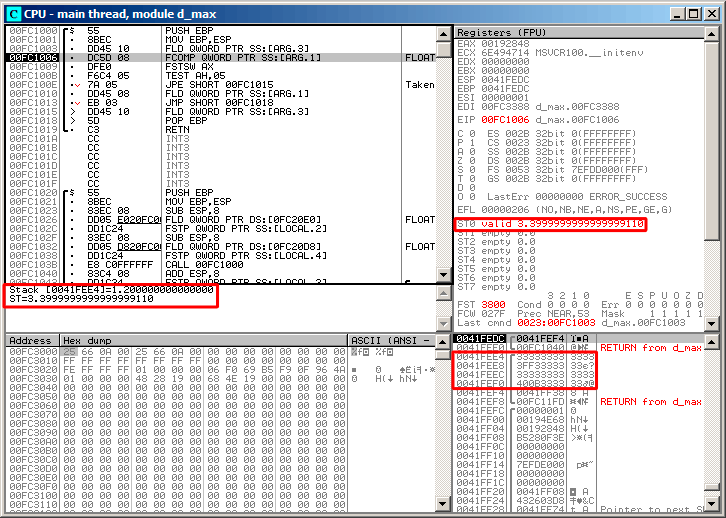
\includegraphics[scale=\FigScale]{patterns/12_FPU/3_comparison/x86/MSVC/olly1_1.png}
\caption{\olly: \RU{первая \FLD исполнилась}\EN{first \FLD is executed}}
\label{fig:FPU_comparison_case1_olly1}
\end{figure}

\RU{Текущие параметры функции: $a=1,2$ и $b=3,4$}\EN{Current arguments of the function: $a=1.2$ and $b=3.4$} 
(\RU{их видно в стеке: 2 пары 32-битных значений}\EN{We can see them in the stack: two pairs of 32-bit values}).
\RU{$b$ (3,4) уже загружено в}\EN{$b$ (3.4) is already loaded in} \ST{0}.
\RU{Сейчас будет исполняться \FCOMP}\EN{Now \FCOMP is being executed}. 
\olly \RU{показывает второй аргумент для \FCOMP, который сейчас находится в стеке}\EN{shows the second \FCOMP
argument, which is in stack right now}.

\clearpage
\FCOMP \RU{отработал}\EN{is executed}:

\begin{figure}[H]
\centering
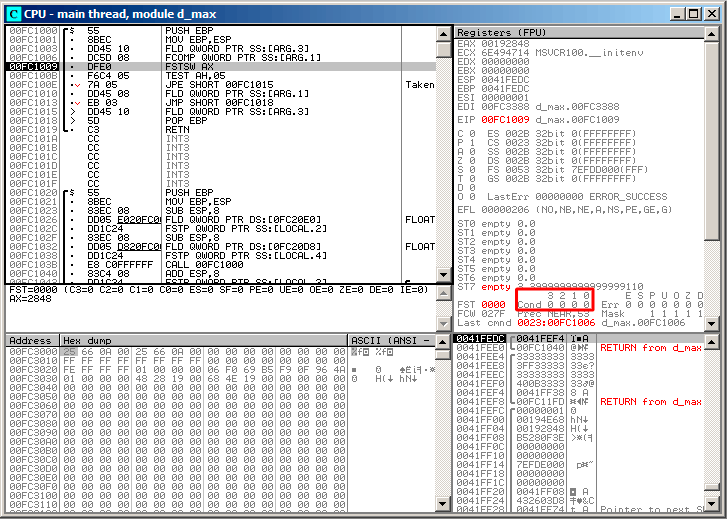
\includegraphics[scale=\FigScale]{patterns/12_FPU/3_comparison/x86/MSVC/olly1_2.png}
\caption{\olly: \FCOMP \RU{исполнилась}\EN{is executed}}
\label{fig:FPU_comparison_case1_olly2}
\end{figure}

\RU{Мы видим состояния condition-флагов \ac{FPU}}\EN{We see the state of the \ac{FPU}'s condition flags}: 
\RU{все нули}\EN{all zeroes}.
\RU{Вытолкнутое значение отображается как \ST{7}. Почему это так, объяснялось ранее}%
\EN{The popped value is reflected as \ST{7}, it was written earlier about reason for this}: 
\myref{FPU_is_rather_circular_buffer}.

\clearpage
\FNSTSW \RU{сработал}\EN{is executed}:
\begin{figure}[H]
\centering
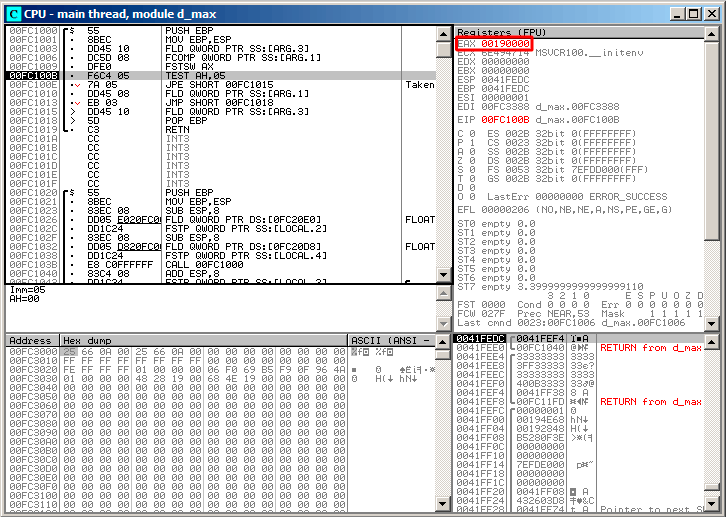
\includegraphics[scale=\FigScale]{patterns/12_FPU/3_comparison/x86/MSVC/olly1_3.png}
\caption{\olly: \FNSTSW \RU{исполнилась}\EN{is executed}}
\label{fig:FPU_comparison_case1_olly3}
\end{figure}

\RU{Видно, что регистр \TT{AX} содержит нули. Действительно, ведь все condition-флаги тоже содержали нули.}
\EN{We see that the \TT{AX} register contain zeroes: indeed, all condition flags are zero.}
(\olly \RU{дизассемблирует команду}\EN{disassembles the} \FNSTSW \RU{как}\EN{instruction as} \TT{FSTSW}\RU{~}---%
\RU{ это синоним}\EN{they are synonyms}).

\clearpage
\TEST \RU{сработал}\EN{is executed}:

\begin{figure}[H]
\centering
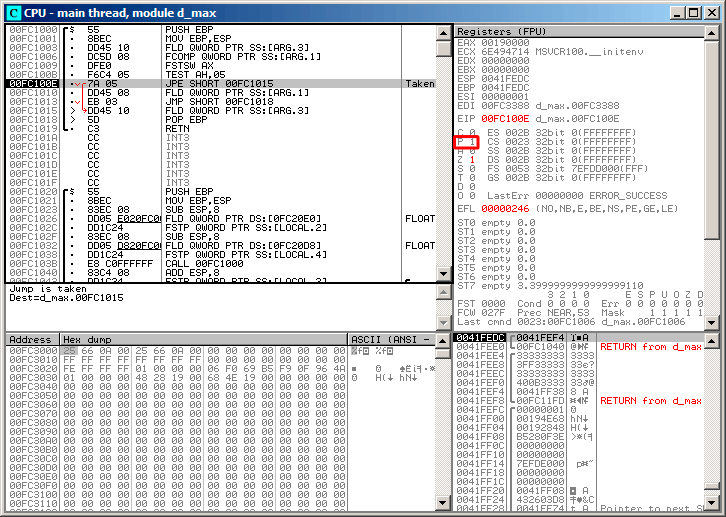
\includegraphics[scale=\FigScale]{patterns/12_FPU/3_comparison/x86/MSVC/olly1_4.png}
\caption{\olly: \TEST \RU{исполнилась}\EN{is executed}}
\label{fig:FPU_comparison_case1_olly4}
\end{figure}

\RU{Флаг \TT{PF} равен единице.}\EN{The \TT{PF} flag is set to 1.}
\RU{Всё верно: количество выставленных бит в 0~--- это 0, а 0~--- это четное число.}
\EN{Indeed: the number of bits set in 0 is 0 and 0 is an even number.}
\olly \RU{дизассемблирует}\EN{disassembles} \TT{JP} \RU{как}\EN{as} \ac{JPE}\RU{~}---\RU{ это синонимы}\EN{they
are synonyms}.
\RU{И она сейчас сработает}\EN{And it is about to trigger now}.

\clearpage
\ac{JPE} \RU{сработала}\EN{triggered}, \FLD \RU{загрузила в \ST{0} значение $b$ (3,4)}%
\EN{loads the value of $b$ (3.4) in \ST{0}}:

\begin{figure}[H]
\centering
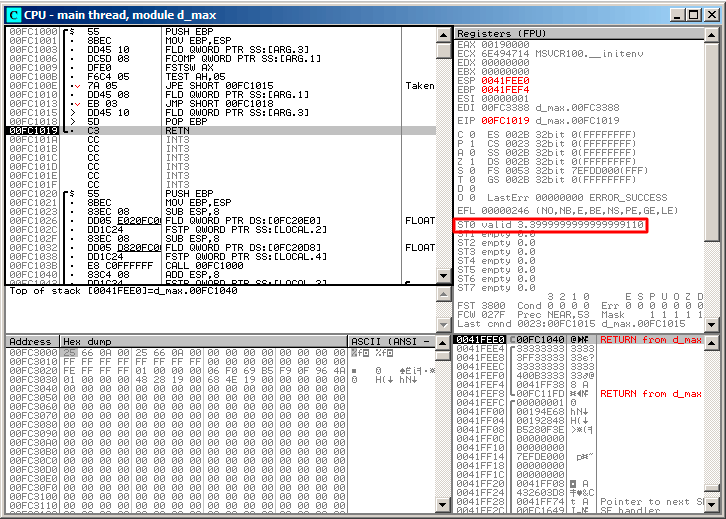
\includegraphics[scale=\FigScale]{patterns/12_FPU/3_comparison/x86/MSVC/olly1_5.png}
\caption{\olly: \RU{вторая \FLD исполнилась}\EN{second \FLD is executed}}
\label{fig:FPU_comparison_case1_olly5}
\end{figure}

\RU{Функция заканчивает свою работу}\EN{The function finishes its work}.

\clearpage
\myparagraph{\RU{Второй пример с \olly: a=5,6 и b=-1}\EN{Second \olly example: a=5.6 and b=-4}}

\RU{Загружаем пример в}\EN{Let's load example into} \olly:

\begin{figure}[H]
\centering
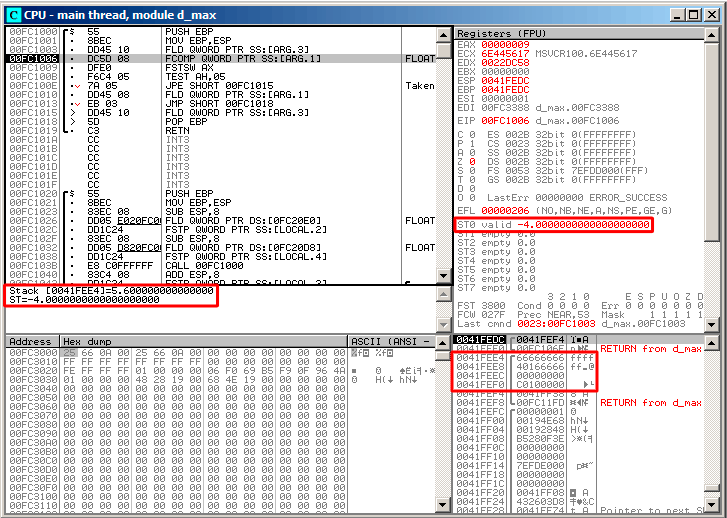
\includegraphics[scale=\FigScale]{patterns/12_FPU/3_comparison/x86/MSVC/olly2_1.png}
\caption{\olly: \RU{первая \FLD исполнилась}\EN{first \FLD executed}}
\label{fig:FPU_comparison_case2_olly1}
\end{figure}

\RU{Текущие параметры функции: $a=5,6$ и $b=-4$}\EN{Current function arguments: $a=5.6$ and $b=-4$}.
$b$ (-4) \RU{уже загружено в}\EN{is already loaded in} \ST{0}.
\RU{Сейчас будет исполняться \FCOMP}\EN{\FCOMP about to execute now}. 
\olly \RU{показывает второй аргумент \FCOMP, который сейчас находится в стеке.}
\EN{shows the second \FCOMP argument, which is in stack right now.}

\clearpage
\FCOMP \RU{отработал}\EN{executed}:

\begin{figure}[H]
\centering
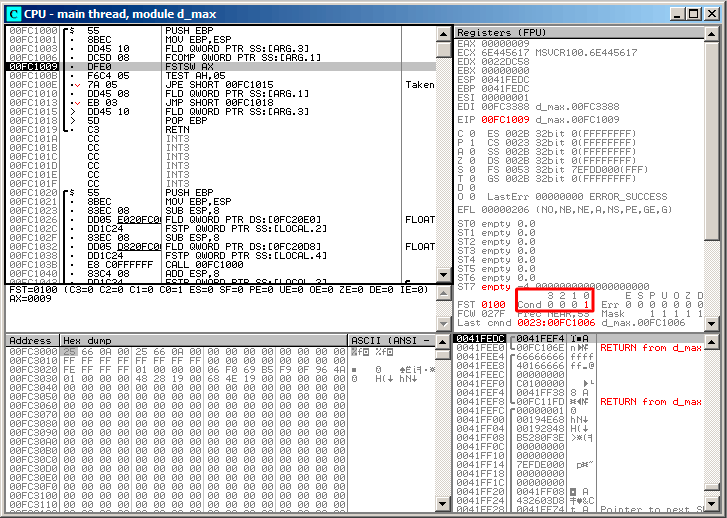
\includegraphics[scale=\FigScale]{patterns/12_FPU/3_comparison/x86/MSVC/olly2_2.png}
\caption{\olly: \FCOMP \RU{исполнилась}\EN{executed}}
\label{fig:FPU_comparison_case2_olly2}
\end{figure}

\RU{Мы видим значения condition-флагов \ac{FPU}: все нули, кроме \Czero.}
\EN{We see the state of the \ac{FPU}'s condition flags: all zeroes except \Czero.}

\clearpage
\FNSTSW \RU{сработал}\EN{executed}:

\begin{figure}[H]
\centering
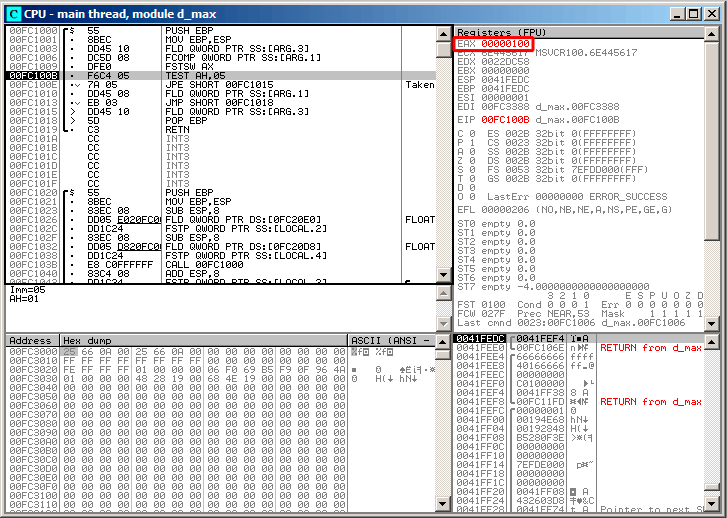
\includegraphics[scale=\FigScale]{patterns/12_FPU/3_comparison/x86/MSVC/olly2_3.png}
\caption{\olly: \FNSTSW \RU{исполнилась}\EN{executed}}
\label{fig:FPU_comparison_case2_olly3}
\end{figure}

\RU{Видно, что регистр \TT{AX} содержит \TT{0x100}: флаг \Czero стал на место 16-го бита.}
\EN{We see that the \TT{AX} register contains \TT{0x100}: the \Czero flag is at the 16th bit.}

\clearpage
\TEST \RU{сработал}\EN{executed}:

\begin{figure}[H]
\centering
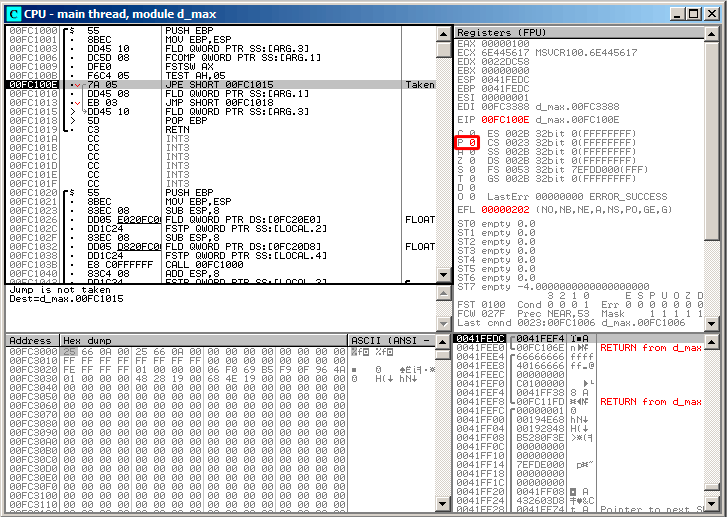
\includegraphics[scale=\FigScale]{patterns/12_FPU/3_comparison/x86/MSVC/olly2_4.png}
\caption{\olly: \TEST \RU{исполнилась}\EN{executed}}
\label{fig:FPU_comparison_case2_olly4}
\end{figure}

\EN{The}\RU{Флаг} \TT{PF} \RU{равен нулю}\EN{ flag is cleared}.
\RU{Всё верно}\EN{Indeed}: 
\RU{количество единичных бит в \TT{0x100}~--- 1, а 1~--- нечетное число.}
\EN{the count of bits set in \TT{0x100} is 1 and 1 is an odd number.}
\ac{JPE} \RU{сейчас не сработает}\EN{is being skipped now}.

\clearpage
\ac{JPE} \RU{не сработала, }\EN{wasn't triggered, so} \FLD 
\RU{загрузила в \ST{0} значение $a$ (5,6)}%
\EN{loads the value of $a$ (5.6) in \ST{0}}:

\begin{figure}[H]
\centering
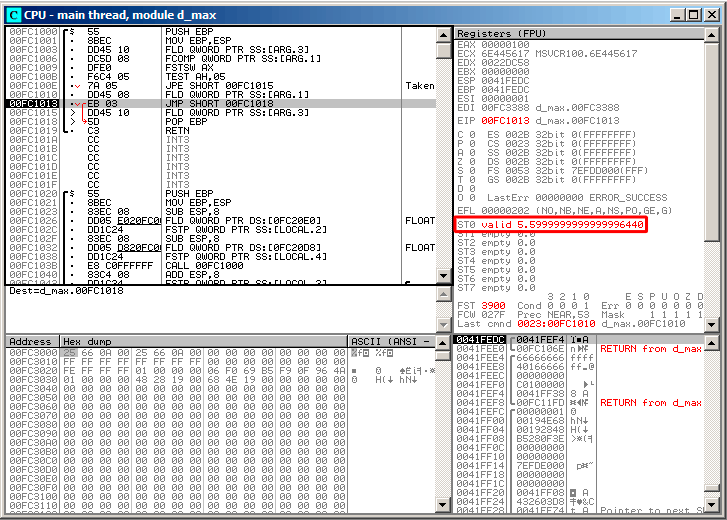
\includegraphics[scale=\FigScale]{patterns/12_FPU/3_comparison/x86/MSVC/olly2_5.png}
\caption{\olly: \RU{вторая \FLD исполнилась}\EN{second \FLD executed}}
\label{fig:FPU_comparison_case2_olly5}
\end{figure}

\RU{Функция заканчивает свою работу}\EN{The function finishes its work}.

\fi

\subsubsection{\Optimizing MSVC 2010}

\lstinputlisting[caption=\Optimizing MSVC 2010]{patterns/12_FPU/3_comparison/x86/MSVC_Ox/MSVC.asm.\LANG}

\index{x86!\Instructions!FCOM}
\RU{\FCOM отличается от \FCOMP тем, что просто сравнивает значения и оставляет стек в том же состоянии. 
В отличие от предыдущего примера, операнды здесь в обратном порядке. 
Поэтому и результат сравнения в \CThreeBits будет отличаться:}
\EN{\FCOM differs from \FCOMP in the sense that it just compares the values and doesn't change the FPU stack. 
Unlike the previous example, here the operands are in reverse order, 
which is why the result of the comparison in \CThreeBits is different:}

\begin{itemize}
\item
\RU{Если $a>b$, то биты \CThreeBits должны быть выставлены так:}
\EN{If $a>b$ in our example, then \CThreeBits bits are to be set as:} 0, 0, 0.
\item
\RU{Если $b>a$, то биты будут выставлены так:}\EN{If $b>a$, then the bits are:} 0, 0, 1.
\item
\RU{Если $a=b$, то биты будут выставлены так:}\EN{If $a=b$, then the bits are:} 1, 0, 0.
\end{itemize}
% TODO: table?

\RU{Инструкция \TT{test ah, 65} как бы оставляет только два бита~--- \Cthree и \Czero. 
Они оба будут нулями, если $a>b$: в таком случае переход \JNE не сработает. 
\index{ARM!\Instructions!FSTP}
Далее имеется инструкция \TT{FSTP ST(1)}~--- эта инструкция копирует 
значение \ST{0} в указанный операнд и выдергивает одно значение из стека. В данном случае, 
она копирует \ST{0} 
(где сейчас лежит~\TT{\_a})~в~\ST{1}. 
После этого на вершине стека два раза лежит~\TT{\_a}. Затем одно значение выдергивается. 
После этого в \ST{0} остается~\TT{\_a} и функция завершается.}
\EN{The \TT{test ah, 65} instruction leaves just two bits~---\Cthree and \Czero. 
Both will be zero if $a>b$: in that case the \JNE jump will not be triggered. 
Then \TT{FSTP ST(1)} follows~---this instruction copies the value from \ST{0} to the operand and 
pops one value from the FPU stack.
In other words, the instruction copies \ST{0} (where the value of \TT{\_a} is now) into \ST{1}.
After that, two copies of {\_a} are at the top of the stack. 
Then, one value is popped.
After that, \ST{0} contains {\_a} and the function is finishes.}

\RU{Условный переход \JNE сработает в двух других случаях: если $b>a$ или $a=b$. 
\ST{0} скопируется в \ST{0} (как бы холостая операция). 
Затем одно значение из стека вылетит и на вершине стека останется то, что 
до этого лежало в \ST{1} (то~есть~\TT{\_b}). И функция завершится. 
Эта инструкция используется здесь видимо потому что в FPU 
нет другой инструкции, которая просто выдергивает 
значение из стека и выбрасывает его.}
\EN{The conditional jump \JNE is triggering in two cases: if $b>a$ or $a=b$. 
\ST{0} is copied into \ST{0}, it is just like an idle (\ac{NOP}) operation, then one value 
is popped from the stack and the top of the stack (\ST{0}) is contain what was in \ST{1} before 
(that is {\_b}). 
Then the function finishes. 
The reason this instruction is used here probably is because the \ac{FPU} 
has no other instruction to pop a value from the stack and discard it.}

\ifdefined\IncludeOlly
\clearpage
\myparagraph{\RU{Первый пример с \olly: a=1,2 и и=3,4}\EN{First \olly example: a=1.2 and b=3.4}}
\index{\olly}

\RU{Обе}\EN{Both} \FLD \RU{отработали}\EN{are executed}:

\begin{figure}[H]
\centering
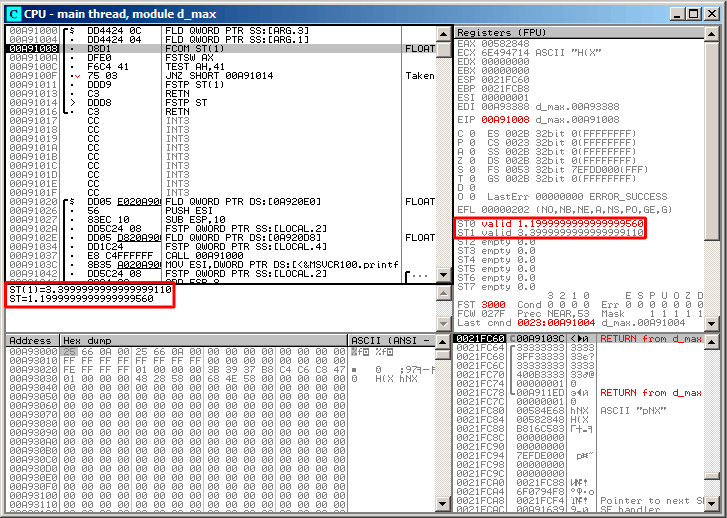
\includegraphics[scale=\FigScale]{patterns/12_FPU/3_comparison/x86/MSVC_Ox/olly1_1.png}
\caption{\olly: \RU{обе \FLD исполнились}\EN{both \FLD are executed}}
\label{fig:FPU_comparison_Ox_case1_olly1}
\end{figure}

\RU{Сейчас будет исполняться }\FCOM\EN{ being executed}: 
\olly \RU{показывает содержимое}\EN{shows the contents of} \ST{0} \AndENRU \ST{1} \RU{для удобства}%
\EN{for convenience}.

\clearpage
\FCOM \RU{сработала}\EN{is done}:

\begin{figure}[H]
\centering
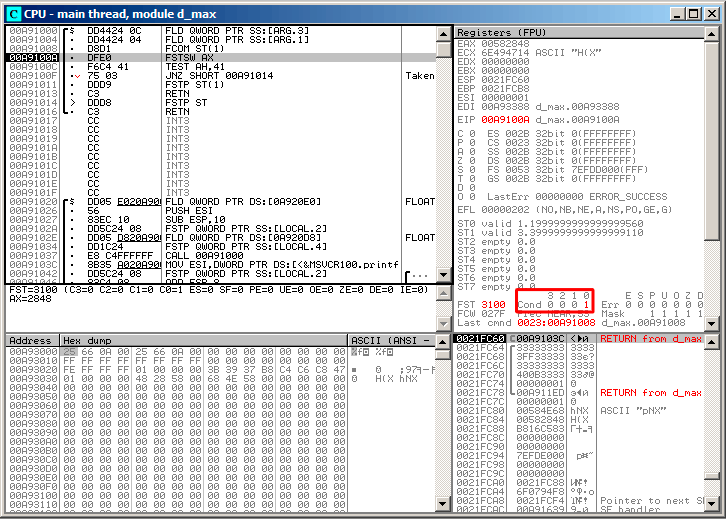
\includegraphics[scale=\FigScale]{patterns/12_FPU/3_comparison/x86/MSVC_Ox/olly1_2.png}
\caption{\olly: \FCOM \RU{исполнилась}\EN{is done}}
\label{fig:FPU_comparison_Ox_case1_olly2}
\end{figure}

\Czero \RU{установлен, остальные флаги сброшены}\EN{is set, all other condition flags are cleared}.

\clearpage
\FNSTSW \RU{сработала}\EN{is done}, \TT{AX}=0x3100:

\begin{figure}[H]
\centering
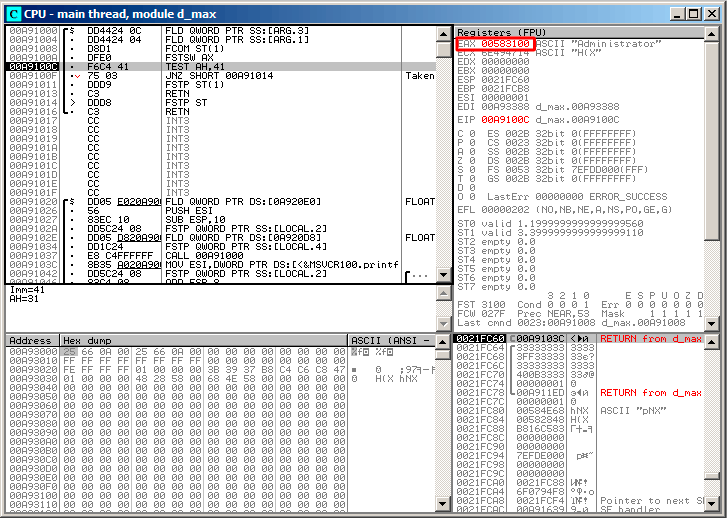
\includegraphics[scale=\FigScale]{patterns/12_FPU/3_comparison/x86/MSVC_Ox/olly1_3.png}
\caption{\olly: \FNSTSW \RU{исполнилась}\EN{is executed}}
\label{fig:FPU_comparison_Ox_case1_olly3}
\end{figure}

\clearpage
\TEST \RU{сработала}\EN{is executed}:

\begin{figure}[H]
\centering
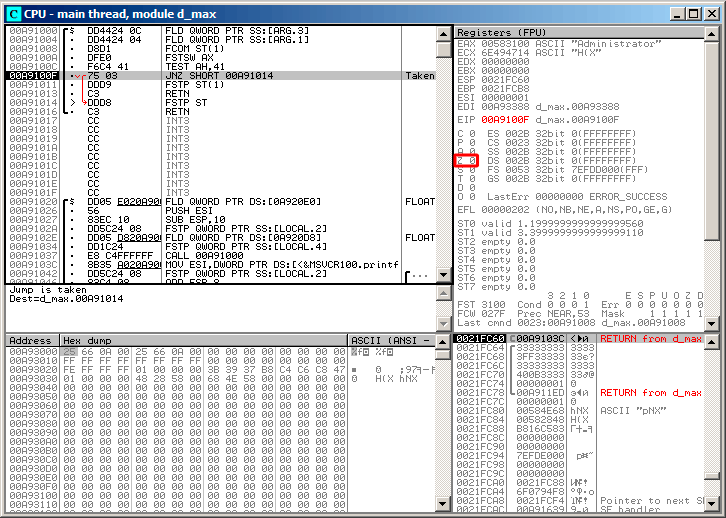
\includegraphics[scale=\FigScale]{patterns/12_FPU/3_comparison/x86/MSVC_Ox/olly1_4.png}
\caption{\olly: \TEST \RU{исполнилась}\EN{is executed}}
\label{fig:FPU_comparison_Ox_case1_olly4}
\end{figure}

ZF=0, \RU{переход сейчас произойдет}\EN{conditional jump is about to trigger now}.

\clearpage
\TT{FSTP ST} (\OrENRU \FSTP \ST{0}) \RU{сработала}\EN{was executed}~---%
\RU{ 1,2 было вытолкнуто из стека, и на вершине осталось 3,4}%
\EN{1.2 was popped from the stack, and 3.4 was left on top}:

\begin{figure}[H]
\centering
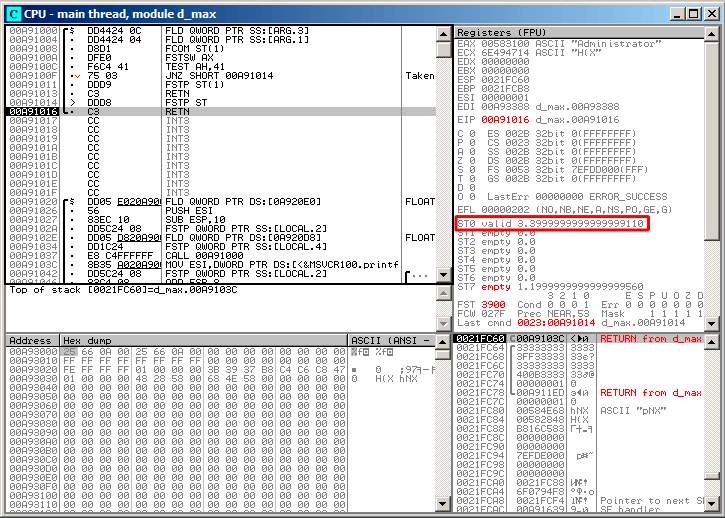
\includegraphics[scale=\FigScale]{patterns/12_FPU/3_comparison/x86/MSVC_Ox/olly1_5.png}
\caption{\olly: \FSTP \RU{исполнилась}\EN{is executed}}
\label{fig:FPU_comparison_Ox_case1_olly5}
\end{figure}

\RU{Видно, что инструкция}\EN{We see that the} \TT{FSTP ST} 
\RU{работает просто как выталкивание одного значения из FPU-стека.}
\EN{instruction works just like popping one value from the FPU stack.}

\clearpage
\myparagraph{\RU{Второй пример с \olly: a=5,6 и b=-4}\EN{Second \olly example: a=5.6 and b=-4}}

\RU{Обе}\EN{Both} \FLD \RU{отработали}\EN{are executed}:

\begin{figure}[H]
\centering
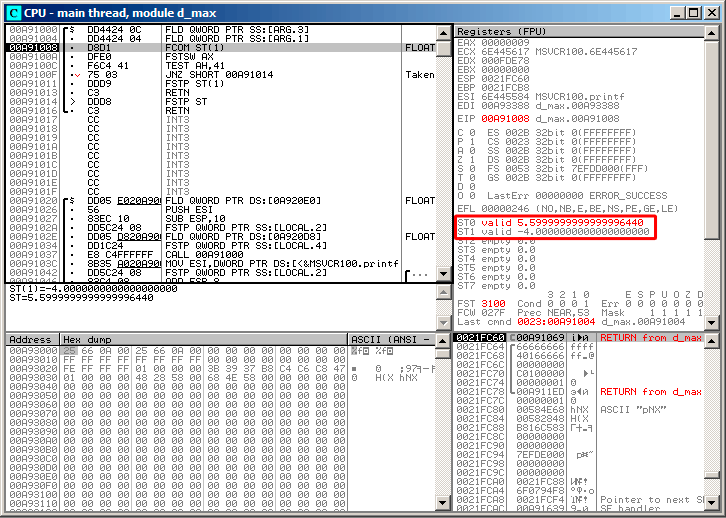
\includegraphics[scale=\FigScale]{patterns/12_FPU/3_comparison/x86/MSVC_Ox/olly2_1.png}
\caption{\olly: \RU{обе \FLD исполнились}\EN{both \FLD are executed}}
\label{fig:FPU_comparison_Ox_case2_olly1}
\end{figure}

\RU{Сейчас будет исполняться \FCOM.}
\EN{\FCOM is about to execute.}

\clearpage
\FCOM \RU{сработала}\EN{is done}:

\begin{figure}[H]
\centering
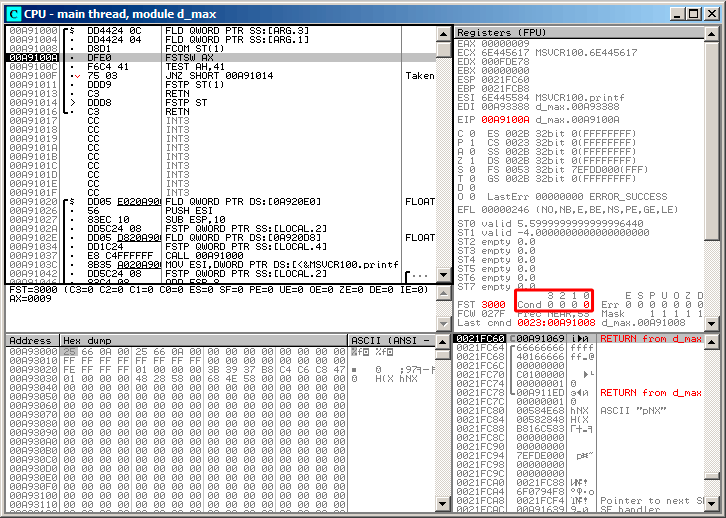
\includegraphics[scale=\FigScale]{patterns/12_FPU/3_comparison/x86/MSVC_Ox/olly2_2.png}
\caption{\olly: \FCOM \RU{исполнилась}\EN{is finished}}
\label{fig:FPU_comparison_Ox_case2_olly2}
\end{figure}

\RU{Все condition-флаги сброшены}\EN{All conditional flags are cleared}.

\clearpage
\FNSTSW \RU{сработала}\EN{done}, \TT{AX}=0x3000:

\begin{figure}[H]
\centering
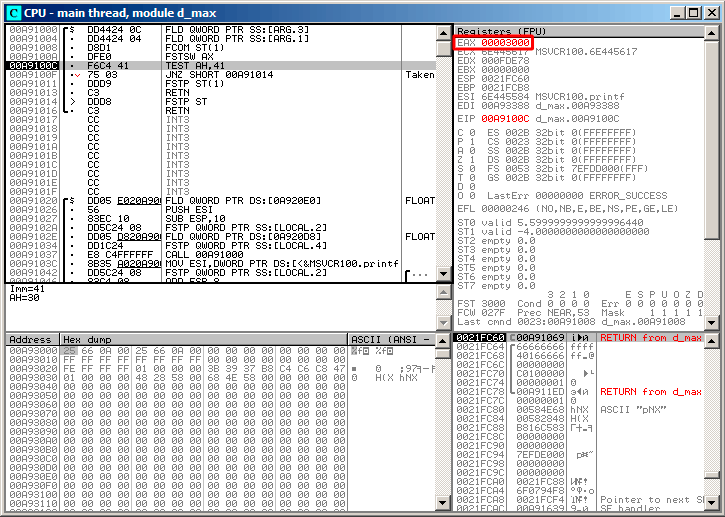
\includegraphics[scale=\FigScale]{patterns/12_FPU/3_comparison/x86/MSVC_Ox/olly2_3.png}
\caption{\olly: \FNSTSW \RU{исполнилась}\EN{was executed}}
\label{fig:FPU_comparison_Ox_case2_olly3}
\end{figure}

\clearpage
\TEST \RU{сработала}\EN{is done}:

\begin{figure}[H]
\centering
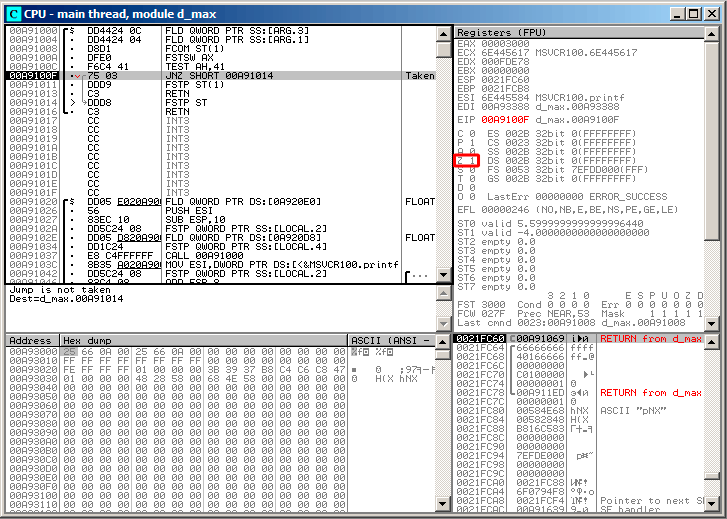
\includegraphics[scale=\FigScale]{patterns/12_FPU/3_comparison/x86/MSVC_Ox/olly2_4.png}
\caption{\olly: \TEST \RU{исполнилась}\EN{was executed}}
\label{fig:FPU_comparison_Ox_case2_olly4}
\end{figure}

ZF=1, \RU{переход сейчас не произойдет}\EN{jump will not happen now}.

\clearpage
\FSTP \ST{1} \RU{сработала: на вершине FPU-стека осталось значение 5,6}\EN{was executed: a value
of 5.6 is now at the top of the FPU stack}.

\begin{figure}[H]
\centering
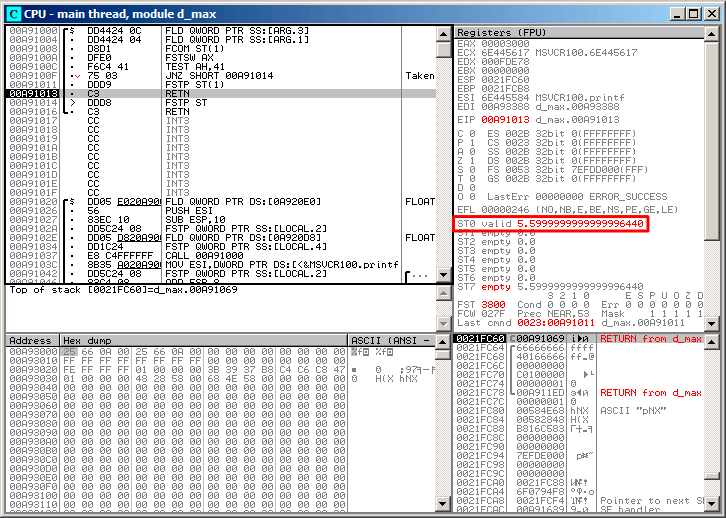
\includegraphics[scale=\FigScale]{patterns/12_FPU/3_comparison/x86/MSVC_Ox/olly2_5.png}
\caption{\olly: \FSTP \RU{исполнилась}\EN{was executed}}
\label{fig:FPU_comparison_Ox_case2_olly5}
\end{figure}

\RU{Видно, что инструкция}\EN{We now see that the} \FSTP \ST{1} 
\RU{работает так: оставляет значение на вершине стека, но обнуляет регистр \ST{1}.}
\EN{instruction works as follows: it leaves what was at the top of the stack, but clears \ST{1}.}

\fi

\ifdefined\IncludeGCC
\subsubsection{GCC 4.4.1}

\lstinputlisting[caption=GCC 4.4.1]{patterns/12_FPU/3_comparison/x86/GCC.asm.\LANG}

\index{x86!\Instructions!FUCOMPP}
\RU{\FUCOMPP~--- это почти то же что и \FCOM, только выкидывает из стека оба значения после сравнения, 
а также несколько иначе реагирует на \q{не-числа}.}
\EN{\FUCOMPP{} is almost like \FCOM, but pops both values from the stack and handles
\q{not-a-numbers} differently.}

\index{\RU{Не-числа}\EN{Non-a-numbers} (NaNs)}
\RU{Немного о \IT{не-числах}}\EN{A bit about \IT{not-a-numbers}}.

\newcommand{\NANFN}{\footnote{\RU{\href{http://go.yurichev.com/17129}{ru.wikipedia.org/wiki/NaN}}%
\EN{\href{http://go.yurichev.com/17130}{wikipedia.org/wiki/NaN}}}}

\RU{FPU умеет работать со специальными переменными, которые числами не являются и называются \q{не числа} или 
\gls{NaN}\NANFN. 
Это бесконечность, результат деления на ноль, и так далее. Нечисла бывают \q{тихие} и \q{сигнализирующие}. 
С первыми можно продолжать работать и далее, а вот если вы попытаетесь совершить какую-то операцию 
с сигнализирующим нечислом, то сработает исключение.}
\EN{The FPU is able to deal with special values which are \IT{not-a-numbers} or 
\gls{NaN}s\NANFN. 
These are infinity, result of division by 0, etc. 
Not-a-numbers can be \q{quiet} and \q{signaling}. It is possible to continue to work with \q{quiet} NaNs, 
but if one tries to do any operation with \q{signaling} NaNs, an exception is to be raised.}

\index{x86!\Instructions!FCOM}
\index{x86!\Instructions!FUCOM}
\RU{Так вот, \FCOM вызовет исключение если любой из операндов какое-либо нечисло.
\FUCOM же вызовет исключение только если один из операндов именно \q{сигнализирующее нечисло}.}
\EN{\FCOM raising an exception if any operand is \gls{NaN}. 
\FUCOM raising an exception only if any operand is a signaling \gls{NaN} (SNaN).}

\index{x86!\Instructions!SAHF}
\label{SAHF}
\RU{Далее мы видим \SAHF (\IT{Store AH into Flags})~--- это довольно редкая инструкция в коде, не использующим FPU. 
8 бит из \AH перекладываются в младшие 8 бит регистра статуса процессора в таком порядке:}
\EN{The next instruction is \SAHF (\IT{Store AH into Flags})~---this is a rare 
instruction in code not related to the FPU. 
8 bits from AH are moved into the lower 8 bits of the CPU flags in the following order:}

\begin{center}
\begin{bytefield}[endianness=big,bitwidth=0.03\linewidth]{8}
\bitheader{7,6,4,2,0} \\
\bitbox{1}{SF} & 
\bitbox{1}{ZF} & 
\bitbox{1}{} & 
\bitbox{1}{AF} & 
\bitbox{1}{} & 
\bitbox{1}{PF} & 
\bitbox{1}{} & 
\bitbox{1}{CF}
\end{bytefield}
\end{center}


\index{x86!\Instructions!FNSTSW}
\RU{Вспомним, что \FNSTSW перегружает интересующие нас биты \CThreeBits в \AH, 
и соответственно они будут в позициях 6, 2, 0 в регистре \AH:}
\EN{Let's recall that \FNSTSW moves the bits that interest us (\CThreeBits) into \AH 
and they are in positions 6, 2, 0 of the \AH register:}

\begin{center}
\begin{bytefield}[endianness=big,bitwidth=0.03\linewidth]{8}
\bitheader{6,2,1,0} \\
\bitbox{1}{} & 
\bitbox{1}{\TT{C3}} & 
\bitbox{3}{} & 
\bitbox{1}{\TT{C2}} & 
\bitbox{1}{\TT{C1}} & 
\bitbox{1}{\TT{C0}}
\end{bytefield}
\end{center}


\RU{Иными словами, пара инструкций \TT{fnstsw  ax / sahf} перекладывает биты \CThreeBits в флаги \ZF, \PF, \CF.}
\EN{In other words, the \TT{fnstsw  ax / sahf} instruction pair moves \CThreeBits into \ZF, \PF and \CF.}

\RU{Теперь снова вспомним, какие значения бит \CThreeBits будут при каких результатах сравнения:}
\EN{Now let's also recall the values of \CThreeBits in different conditions:}

\begin{itemize}
\item
\RU{Если $a$ больше $b$ в нашем случае, то биты \CThreeBits должны быть выставлены так:}
\EN{If $a$ is greater than $b$ in our example, then \CThreeBits are to be set to:} 0, 0, 0.
\item
\RU{Если $a$ меньше $b$, то биты будут выставлены так:}
\EN{if $a$ is less than $b$, then the bits are to be set to:} 0, 0, 1.
\item
\RU{Если $a=b$, то так:}\EN{If $a=b$, then:} 1, 0, 0.
\end{itemize}
% TODO: table?

\RU{Иными словами, после трех инструкций \FUCOMPP/\FNSTSW/\SAHF 
возможны такие состояния флагов:}
\EN{In other words, these states of the CPU flags are possible
after three \FUCOMPP/\FNSTSW/\SAHF instructions:}

\begin{itemize}
\item
\RU{Если $a>b$ в нашем случае, то флаги будут выставлены так:}
\EN{If $a>b$, the CPU flags are to be set as:} \TT{ZF=0, PF=0, CF=0}.
\item
\RU{Если $a<b$, то флаги будут выставлены так:}
\EN{If $a<b$, then the flags are to be set as:} \TT{ZF=0, PF=0, CF=1}.
\item
\RU{Если $a=b$, то так:}\EN{And if $a=b$, then:} \TT{ZF=1, PF=0, CF=0}.
\end{itemize}
% TODO: table?

\index{x86!\Instructions!SETcc}
\index{x86!\Instructions!JNBE}
\RU{Инструкция \SETNBE выставит в \AL единицу или ноль в зависимости от флагов и условий. 
Это почти аналог \JNBE, за тем лишь исключением, что \SETcc
\footnote{\IT{cc} это \IT{condition code}}
выставляет 1 или 0 в \AL, а \Jcc делает переход или нет. 
\SETNBE запишет 1 только если \TT{CF=0} и \TT{ZF=0}. Если это не так, то запишет 0 в \AL.}
\EN{Depending on the CPU flags and conditions, \SETNBE stores 1 or 0 to AL. 
It is almost the counterpart of \JNBE, with the exception that \SETcc 
\footnote{\IT{cc} is \IT{condition code}} stores 1 or 0 in \AL, 
but \Jcc does actually jump or not. 
\SETNBE stores 1 only if \TT{CF=0} and \TT{ZF=0}. 
If it is not true, 0 is to be stored into \AL.}

\RU{\CF будет 0 и \ZF будет 0 одновременно только в одном случае: если $a>b$.}
\EN{Only in one case both \CF and \ZF are 0: if $a>b$.}

\RU{Тогда в \AL будет записана 1, последующий условный переход \JZ выполнен не будет 
и функция вернет~\TT{\_a}. 
В остальных случаях, функция вернет~\TT{\_b}.}
\EN{Then 1 is to be stored to \AL, 
the subsequent \JZ is not to be triggered and the function will return {\_a}. 
In all other cases, {\_b} is to be returned.}
\fi

\subsubsection{\Optimizing GCC 4.4.1}

\lstinputlisting[caption=\Optimizing GCC 4.4.1]{patterns/12_FPU/3_comparison/x86/GCC_O3.asm.\LANG}

\index{x86!\Instructions!JA}
\RU{Почти всё что здесь есть, уже описано мною, кроме одного: использование \JA после \SAHF. 
Действительно, инструкции условных переходов \q{больше}, \q{меньше} и \q{равно} для сравнения беззнаковых чисел 
(а это \JA, \JAE, \JB, \JBE, \JE/\JZ, \JNA, \JNAE, \JNB, \JNBE, \JNE/\JNZ) проверяют только флаги \CF и \ZF.}
\EN{It is almost the same except that \JA is used after \SAHF. 
Actually, conditional jump instructions that check \q{larger}, \q{lesser} or \q{equal} for unsigned number comparison 
(these are \JA, \JAE, \JB, \JBE, \JE/\JZ, \JNA, \JNAE, \JNB, \JNBE, \JNE/\JNZ) check only flags \CF and \ZF.}\ESph{}\PTBRph{}\PLph{}\\
\\
\EN{Let's recall where bits \CThreeBits are located in the \TT{AH} register after the execution of \TT{FSTSW}/\FNSTSW:}
\RU{Вспомним, как биты \CThreeBits располагаются в регистре \TT{AH} после исполнения \TT{FSTSW}/\FNSTSW:}

\begin{center}
\begin{bytefield}[endianness=big,bitwidth=0.03\linewidth]{8}
\bitheader{6,2,1,0} \\
\bitbox{1}{} & 
\bitbox{1}{\TT{C3}} & 
\bitbox{3}{} & 
\bitbox{1}{\TT{C2}} & 
\bitbox{1}{\TT{C1}} & 
\bitbox{1}{\TT{C0}}
\end{bytefield}
\end{center}


\RU{Вспомним также, как располагаются биты из \TT{AH} во флагах CPU после исполнения \SAHF:}
\EN{Let's also recall, how the bits from \TT{AH} are stored into the CPU flags the execution of \SAHF:}

\begin{center}
\begin{bytefield}[endianness=big,bitwidth=0.03\linewidth]{8}
\bitheader{7,6,4,2,0} \\
\bitbox{1}{SF} & 
\bitbox{1}{ZF} & 
\bitbox{1}{} & 
\bitbox{1}{AF} & 
\bitbox{1}{} & 
\bitbox{1}{PF} & 
\bitbox{1}{} & 
\bitbox{1}{CF}
\end{bytefield}
\end{center}


\RU{Биты \Cthree и \Czero после сравнения перекладываются в флаги \ZF и \CF так, 
что перечисленные инструкции переходов могут работать. 
\JA сработает, если \CF и \ZF обнулены.}
\EN{After the comparison, the \Cthree and \Czero bits are moved into \ZF and \CF,
so the conditional jumps are able work after.
\JA is triggering if both \CF are \ZF zero.}

\RU{Таким образом, перечисленные инструкции условного перехода можно использовать после инструкций \FNSTSW/\SAHF.}
\EN{Thereby, the conditional jumps instructions listed here can be used after a \FNSTSW/\SAHF instruction pair.}

\RU{Может быть, биты статуса FPU \CThreeBits преднамеренно были размещены таким образом, 
чтобы переноситься на базовые флаги процессора без перестановок?}
\EN{Apparently, the FPU \CThreeBits status bits were placed there intentionally, 
to easily map them to base CPU flags without additional permutations?}

\ifdefined\IncludeGCC
\subsubsection{GCC 4.8.1 \RU{с оптимизацией \Othree}\EN{with \Othree optimization turned on}}
\label{gcc481_o3}

\EN{Some new FPU instructions were added in the P6 Intel family}\RU{В линейке процессоров P6 от Intel 
появились новые FPU-инструкции}\footnote{\EN{Starting at}\RU{Начиная с} Pentium Pro, 
Pentium-II, \etc.}.
\index{x86!\Instructions!FUCOMI}
\RU{Это}\EN{These are} \TT{FUCOMI} (\RU{сравнить операнды и выставить флаги основного CPU}\EN{compare 
operands and set flags of the main CPU}) \AndENRU 
\index{x86!\Instructions!FCMOVcc}
\TT{FCMOVcc} (\RU{работает как}\EN{works like} \TT{CMOVcc}, \RU{но на регистрах FPU}\EN{but on FPU registers}).
\RU{Очевидно, разработчики GCC решили отказаться от поддержки процессоров до линейки P6 (ранние Pentium, 80486, etc{}.)}
\EN{Apparently, the maintainers of GCC decided to drop support of pre-P6 Intel CPUs (early Pentiums, 80486, etc{})}.

\RU{И кстати, FPU уже давно не отдельная часть процессора в линейке P6, так что флаги основного CPU можно
модифицировать из FPU.}
\EN{And also, the FPU is no longer separate unit in P6 Intel family, so now it is possible to modify/check flags 
of the main CPU from the FPU.}

\RU{Вот что имеем}\EN{So what we get is}:

\lstinputlisting[caption=\Optimizing GCC 4.8.1]{patterns/12_FPU/3_comparison/x86/GCC481_O3.s.\LANG}

\RU{Не совсем понимаю, зачем здесь \TT{FXCH} (поменять местами операнды).}
\EN{Hard to guess why \TT{FXCH} (swap operands) is here.}
\RU{От нее легко избавиться поменяв местами инструкции \FLD либо заменив 
\TT{FCMOVBE} (\IT{below or equal}~--- меньше или равно) на 
\TT{FCMOVA} (\IT{above}~--- больше).}
\EN{It's possible to get rid of it easily by swapping the first two \FLD instructions or by replacing 
\TT{FCMOVBE} (\IT{below or equal}) by \TT{FCMOVA} (\IT{above}).}
\RU{Должно быть, неаккуратность компилятора}\EN{Probably it's a compiler inaccuracy}.

\RU{Так что}\EN{So} \TT{FUCOMI} \EN{compares}\RU{сравнивает} \ST{0} ($a$) \AndENRU \ST{1} ($b$) 
\RU{и затем устанавливает флаги основного CPU}\EN{and then sets some flags in the main CPU}.
\TT{FCMOVBE} \RU{проверяет флаги и копирует}\EN{checks the flags and copies} \ST{1} 
(\RU{в тот момент там находится $b$}\EN{$b$ here at the moment}) \RU{в}\EN{to} 
\ST{0} (\RU{там $a$}\EN{$a$ here}) \RU{если}\EN{if} $ST0 (a) <= ST1 (b)$.
\RU{В противном случае}\EN{Otherwise} ($a>b$), \RU{она оставляет}\EN{it leaves} $a$ \InENRU \ST{0}.

\RU{Последняя}\EN{The last} \FSTP \RU{оставляет содержимое}\EN{leaves} \ST{0} 
\RU{на вершине стека, выбрасывая содержимое}\EN{on top of the stack, discarding the contents of} \ST{1}.

\ifdefined\IncludeGDB
\RU{Попробуем оттрасировать функцию в}\EN{Let's trace this function in} GDB:

\lstinputlisting[caption=\Optimizing GCC 4.8.1 and GDB,numbers=left]{patterns/12_FPU/3_comparison/x86/gdb.txt}

\RU{Используя}\EN{Using} \q{ni}, \RU{дадим первым двум инструкциям \FLD исполниться.}
\EN{let's execute the first two \FLD instructions.}

\RU{Посмотрим регистры FPU}\EN{Let's examine the FPU registers} (\LineENRU 33).

\RU{Как уже было указано ранее, регистры FPU это скорее кольцевой буфер, нежели стек}%
\EN{As it was mentioned before, the FPU registers set is a circular buffer rather than a stack} (\myref{FPU_is_rather_circular_buffer}).
\RU{И}\EN{And} GDB \RU{показывает не регистры}\EN{doesn't show} \TT{STx}\RU{, а внутренние регистры FPU}
\EN{registers, but internal the FPU registers} (\TT{Rx}). 
\RU{Стрелка}\EN{The arrow} (\RU{на строке}\EN{at line} 35) 
\RU{указывает на текущую вершину стека.}
\EN{points to the current top of the stack.}
\RU{Вы можете также увидеть содержимое регистра \TT{TOP} в \q{Status Word} (строка 44). Там сейчас 6, так что
вершина стека сейчас указывает на внутренний регистр 6.}
\EN{You can also see the \TT{TOP} register contents in \IT{Status Word} (line 44)---it is 6 now, 
so the stack top is now pointing to internal register 6.}

\RU{Значения $a$ и $b$ меняются местами после исполнения \TT{FXCH}}\EN{The values of $a$ and $b$ are swapped 
after \TT{FXCH} is executed} (\LineENRU 54).

\TT{FUCOMI} \RU{исполнилась}\EN{is executed} (\LineENRU 83). 
\RU{Посмотрим флаги}\EN{Let's see the flags}: \CF \RU{выставлен}\EN{is set} (\LineENRU 95).

\TT{FCMOVBE} \RU{действительно скопировал значение $b$ (см. строку 104).}
\EN{has copied the value of $b$ (see line 104).}

\FSTP \RU{оставляет одно значение на вершине стека}\EN{leaves one value at the top of stack} (\LineENRU 136). 
\RU{Значение \TT{TOP} теперь 7, так что вершина FPU-стека указывает на внутренний регистр 7}\EN{The value of \TT{TOP} is 
now 7, so the FPU stack top is pointing to internal register 7}.
\fi
\fi


\ifdefined\IncludeARM
\subsection{ARM}

\subsubsection{\OptimizingXcodeIV (\ARMMode)}

\lstinputlisting[caption=\OptimizingXcodeIV (\ARMMode)]{patterns/12_FPU/3_comparison/ARM/Xcode_ARM.lst.\LANG}

\index{ARM!\Registers!APSR}
\index{ARM!\Registers!FPSCR}
\RU{Очень простой случай.}\EN{A very simple case.}
\RU{Входные величины помещаются в}\EN{The input values are placed into the} \TT{D17} \AndENRU \TT{D16} 
\RU{и сравниваются при помощи инструкции}\EN{registers and then compared using the} 
\TT{VCMPE}\EN{ instruction}.
\RU{Как и в сопроцессорах x86, сопроцессор в ARM имеет свой собственный регистр статуса и флагов}%
\EN{Just like in the x86 coprocessor, the ARM coprocessor has its own status and flags register} (\ac{FPSCR}),
\RU{потому что есть необходимость хранить специфичные для его работы флаги.}
\EN{since there is a need to store coprocessor-specific flags.}
% TODO -> расписать регистр по битам
\index{ARM!\Instructions!VMRS}
\RU{И так же, как и в x86}\EN{And just like in x86}, 
\RU{в ARM нет инструкций условного перехода}%
\EN{there are no conditional jump instruction in ARM}, 
\RU{проверяющих биты в регистре статуса сопроцессора}\EN{that can check bits in the status register of the coprocessor}. 
\RU{Поэтому имеется инструкция}\EN{So there is} \TT{VMRS}%
\RU{, копирующая 4 бита}\EN{, which copies 4 bits} (N, Z, C, V) 
\RU{из статуса сопроцессора в биты \IT{общего} статуса (регистр \ac{APSR}).}
\EN{from the coprocessor status word into bits of the \IT{general} status register (\ac{APSR}).}

\index{ARM!\Instructions!VMOVGT}
\TT{VMOVGT} \RU{это аналог}\EN{is the analog of the} \TT{MOVGT}, 
\RU{инструкция для D-регистров, срабатывающая, если при сравнении один операнд был больше чем второй}
\EN{instruction for D-registers, it executes if one operand is greater than the other while comparing} 
(\IT{GT\EMDASH{}Greater Than}). 

\RU{Если она сработает}\EN{If it gets executed}, 
\RU{в \TT{D16} запишется значение $b$}\EN{the value of $b$ is to be written into \TT{D16}}%
\RU{, лежащее в тот момент в}\EN{(that is currently stored in in} \TT{D17}\EN{)}.

\RU{В обратном случае}\EN{Otherwise} 
\RU{в \TT{D16} остается значение $a$.}
\EN{the value of $a$ stays in the \TT{D16} register.}

\index{ARM!\Instructions!VMOV}
\RU{Предпоследняя инструкция \TT{VMOV} готовит то, что было в \TT{D16}, для возврата через 
пару регистров \Reg{0} и \Reg{1}.}
\EN{The penultimate instruction \TT{VMOV} prepares the value in the \TT{D16} register for returning it via the \Reg{0} and \Reg{1}
register pair.}

\subsubsection{\OptimizingXcodeIV (\ThumbTwoMode)}

\begin{lstlisting}[caption=\OptimizingXcodeIV (\ThumbTwoMode)]
VMOV            D16, R2, R3 ; b
VMOV            D17, R0, R1 ; a
VCMPE.F64       D17, D16
VMRS            APSR_nzcv, FPSCR
IT GT 
VMOVGT.F64      D16, D17
VMOV            R0, R1, D16
BX              LR
\end{lstlisting}

\RU{Почти то же самое, что и в предыдущем примере, за парой отличий.}
\EN{Almost the same as in the previous example, however slightly different.}
\RU{Как мы уже знаем, многие инструкции в режиме ARM можно дополнять условием.}
\EN{As we already know, many instructions in ARM mode can be supplemented by condition predicate.}

\RU{Но в режиме Thumb такого нет.}
\EN{But there is no such thing in Thumb mode.} 
\RU{В 16-битных инструкций просто нет места для лишних 4 битов, при помощи
которых можно было бы закодировать условие выполнения.}
\EN{There is no space in the 16-bit instructions for 4 more bits in which conditions can be encoded.}

\index{ARM!\ThumbTwoMode}
\RU{Поэтому в Thumb-2 добавили возможность дополнять Thumb-инструкции условиями.}
\EN{However, Thumb-2 was extended to make it possible to specify predicates to old Thumb instructions.}

\RU{В листинге, сгенерированном при помощи \IDA, мы видим инструкцию \TT{VMOVGT}, 
такую же как и в предыдущем примере.}
\EN{Here, in the \IDA-generated listing, we see the \TT{VMOVGT} instruction, as in previous example.}

\RU{В реальности}\EN{In fact,} 
\RU{там закодирована обычная инструкция \TT{VMOV}}%
\EN{the usual \TT{VMOV} is encoded there}, 
\RU{просто \IDA добавила суффикс \TT{-GT} к ней}%
\EN{but \IDA adds the \TT{-GT} suffix to it}, 
\RU{потому что перед этой инструкцией стоит \TT{IT GT}.}
\EN{since there is a \TT{\q{IT GT}} instruction placed right before it.}

\label{ARM_Thumb_IT}
\index{ARM!\Instructions!IT}
\index{ARM!if-then block}
\EN{The}\RU{Инструкция} \TT{IT} \RU{определяет так называемый}\EN{instruction defines a so-called} \IT{if-then block}. 
\RU{После этой инструкции можно указывать до четырех инструкций, 
к каждой из которых будет добавлен суффикс условия.}
\EN{After the instruction it is possible to place up to 4 instructions, 
each of them has a predicate suffix.}
\RU{В нашем примере}\EN{In our example,} \TT{IT GT} \RU{означает,}\EN{implies}
\RU{что следующая за ней инструкция будет исполнена, если условие}
\EN{that the next instruction is to be executed, if the}
\IT{GT} (\IT{Greater Than}) \RU{справедливо}\EN{condition is true}.

\index{Angry Birds}
\RU{Теперь более сложный пример. Кстати, из}\EN{Here is a more complex code fragment, by the way, from} 
Angry Birds (\RU{для}\EN{for} iOS):

% FIXME russian listing:
\begin{lstlisting}[caption=Angry Birds Classic]
...
ITE NE
VMOVNE          R2, R3, D16
VMOVEQ          R2, R3, D17
BLX             _objc_msgSend ; not prefixed
...
\end{lstlisting}

\TT{ITE} \RU{означает}\EN{stands for} \IT{if-then-else} 
\RU{и кодирует суффиксы для двух следующих за ней инструкций.}
\EN{and it encodes suffixes for the next two instructions.}
\RU{Первая из них исполнится, если условие, закодированное в}
\EN{The first instruction executes if the condition encoded in} \TT{ITE} (\IT{NE, not equal}) 
\RU{будет в тот момент справедливо}\EN{is true at},
\RU{а вторая~--- если это условие не сработает}\EN{and the 
second---if the condition is not true}.
(\RU{Обратное условие от}\EN{The inverse condition of} \TT{NE} \RU{это}\EN{is} \TT{EQ} (\IT{equal})).

\EN{The instruction followed after the second VMOV (or VMOVEQ) is a normal one, not prefixed (BLX).}
\RU{Инструкция следующая за второй VMOV (или VMOEQ) нормальная, без префикса (BLX).}

\index{Angry Birds}
\RU{Ещё чуть сложнее}\EN{One more that's slightly harder}, 
\RU{и снова этот фрагмент из}\EN{which is also from} Angry Birds:

% FIXME russian listing:
\begin{lstlisting}[caption=Angry Birds Classic]
...
ITTTT EQ
MOVEQ           R0, R4
ADDEQ           SP, SP, #0x20
POPEQ.W         {R8,R10}
POPEQ           {R4-R7,PC}
BLX             ___stack_chk_fail ; not prefixed
...
\end{lstlisting}

\RU{Четыре символа \q{T} в инструкции означают, что четыре последующие инструкции будут исполнены если условие соблюдается.}
\EN{Four \q{T} symbols in the instruction mnemonic mean 
that the four subsequent instructions are to be executed if the condition is true.}
\RU{Поэтому \IDA добавила ко всем четырем инструкциям суффикс}
\EN{That's why \IDA adds the} \TT{-EQ}\EN{ suffix
to each one of them}. 

\RU{А если бы здесь было, например,}\EN{And if there was be, for example,}
\TT{ITEEE EQ} (\IT{if-then-else-else-else}), 
\RU{тогда суффиксы для следующих четырех инструкций были бы расставлены так:}
\EN{then the suffixes would have been set as follows:}

\begin{lstlisting}
-EQ
-NE
-NE
-NE
\end{lstlisting}

\index{Angry Birds}
\RU{Ещё фрагмент из}\EN{Another fragment from} Angry Birds:

% FIXME russian listing:
\begin{lstlisting}[caption=Angry Birds Classic]
...
CMP.W           R0, #0xFFFFFFFF
ITTE LE
SUBLE.W         R10, R0, #1
NEGLE           R0, R0
MOVGT           R10, R0
MOVS            R6, #0         ; not prefixed
CBZ             R0, loc_1E7E32 ; not prefixed
...
\end{lstlisting}

\TT{ITTE} (\IT{if-then-then-else}) 
\RU{означает, что первая и вторая инструкции исполнятся, если условие \TT{LE} (\IT{Less or Equal})
справедливо, а третья~--- если справедливо обратное условие (\TT{GT}\EMDASH\IT{Greater Than}).}
\EN{implies that the 1st and 2nd instructions are to be executed if the \TT{LE} (\IT{Less or Equal})
condition is true, and the 3rd---if the inverse condition (\TT{GT}\EMDASH\IT{Greater Than}) 
is true.}

\RU{Компиляторы способны генерировать далеко не все варианты.}
\EN{Compilers usually don't generate all possible combinations.}
\index{Angry Birds}
\RU{Например, в вышеупомянутой игре Angry Birds (версия \IT{classic} для iOS)}
\EN{For example, in the mentioned Angry Birds game (\IT{classic} version for iOS)}
\RU{встречаются только такие варианты инструкции \TT{IT}}\EN{only these variants of the \TT{IT} instruction are used}: 
\TT{IT}, \TT{ITE}, \TT{ITT}, \TT{ITTE}, \TT{ITTT}, \TT{ITTTT}.
\index{\GrepUsage}
\RU{Как это узнать?}\EN{How to learn this?}
\RU{В \IDA можно сгенерировать листинг (что и было сделано), только в опциях был установлен показ 4 байтов для каждого опкода.}
\EN{In \IDA It is possible to produce listing files, so it was created with an option to show 4 bytes for each opcode.}
\RU{Затем, зная что старшая часть 16-битного опкода (\TT{IT} это \TT{0xBF}), сделаем при помощи \TT{grep} это:}
\EN{Then, knowing the high part of the 16-bit opcode (\TT{IT} is \TT{0xBF}), we do the following using \TT{grep}:}

\begin{lstlisting}
cat AngryBirdsClassic.lst | grep " BF" | grep "IT" > results.lst
\end{lstlisting}

\index{ARM!\ThumbTwoMode}
\RU{Кстати, если писать на ассемблере для режима Thumb-2 вручную, и дополнять инструкции суффиксами
условия, то ассемблер автоматически будет добавлять инструкцию \TT{IT} с соответствующими флагами там,
где надо.}
\EN{By the way, if you program in ARM assembly language manually for Thumb-2 mode, 
and you add conditional suffixes,
the assembler will add the \TT{IT} instructions automatically with the required flags where it is necessary.}

\subsubsection{\NonOptimizingXcodeIV (\ARMMode)}

\begin{lstlisting}[caption=\NonOptimizingXcodeIV (\ARMMode)]
b               = -0x20
a               = -0x18
val_to_return   = -0x10
saved_R7        = -4

                STR             R7, [SP,#saved_R7]!
                MOV             R7, SP
                SUB             SP, SP, #0x1C
                BIC             SP, SP, #7
                VMOV            D16, R2, R3
                VMOV            D17, R0, R1
                VSTR            D17, [SP,#0x20+a]
                VSTR            D16, [SP,#0x20+b]
                VLDR            D16, [SP,#0x20+a]
                VLDR            D17, [SP,#0x20+b]
                VCMPE.F64       D16, D17
                VMRS            APSR_nzcv, FPSCR
                BLE             loc_2E08
                VLDR            D16, [SP,#0x20+a]
                VSTR            D16, [SP,#0x20+val_to_return]
                B               loc_2E10

loc_2E08
                VLDR            D16, [SP,#0x20+b]
                VSTR            D16, [SP,#0x20+val_to_return]

loc_2E10
                VLDR            D16, [SP,#0x20+val_to_return]
                VMOV            R0, R1, D16
                MOV             SP, R7
                LDR             R7, [SP+0x20+b],#4
                BX              LR
\end{lstlisting}

\RU{Почти то же самое, что мы уже видели}\EN{Almost the same as we already saw}, 
\RU{но много избыточного кода из-за хранения $a$ и $b$, 
а также выходного значения, в локальном стеке.}
\EN{but there is too much redundant code because the $a$ and $b$ variables are stored in the local stack, as well
as the return value.}

\subsubsection{\OptimizingKeilVI (\ThumbMode)}

\begin{lstlisting}[caption=\OptimizingKeilVI (\ThumbMode)]
                PUSH    {R3-R7,LR}
                MOVS    R4, R2
                MOVS    R5, R3
                MOVS    R6, R0
                MOVS    R7, R1
                BL      __aeabi_cdrcmple
                BCS     loc_1C0
                MOVS    R0, R6
                MOVS    R1, R7
                POP     {R3-R7,PC}

loc_1C0
                MOVS    R0, R4
                MOVS    R1, R5
                POP     {R3-R7,PC}
\end{lstlisting}

\RU{Keil не генерирует FPU-инструкции, потому что не 
рассчитывает на то, что они будет поддерживаться, а простым сравнением побитово здесь не обойтись.}
\EN{Keil doesn't generate FPU-instructions since it cannot rely on them being
supported on the target CPU, and it cannot be done by straightforward bitwise comparing.}
%TODO1: why?
\RU{Для сравнения вызывается библиотечная функция}\EN{So it calls an external library
function to do the comparison:} \TT{\_\_aeabi\_cdrcmple}. 
\index{ARM!\Instructions!BCS}\\
\\
N.B. \RU{Результат
сравнения эта функция оставляет в флагах, чтобы следующая за вызовом инструкция}
\EN{The result of the comparison is to be left in the flags by this function, so the following}
\TT{BCS} (\IT{Carry set\RU{~}---\RU{ }Greater than or equal})
\RU{могла работать без дополнительного кода.}\EN{instruction can work without any additional code.}

\subsection{ARM64}

\subsubsection{\Optimizing GCC (Linaro) 4.9}

\lstinputlisting{patterns/12_FPU/3_comparison/ARM/ARM64_GCC_O3.lst.\LANG}

\EN{The}\RU{В} ARM64 \ac{ISA} \RU{теперь есть FPU-инструкции, устанавливающие флаги CPU}\EN{has FPU-instructions 
which set} \ac{APSR} \RU{вместо}\EN{the CPU flags instead of} \ac{FPSCR} \EN{for convenience}\RU{для удобства}.
\EN{The}\ac{FPU} \RU{больше не отдельное устройство (по крайней мере логически)}\EN{is not a separate device here 
anymore (at least, logically)}.
\index{ARM!\Instructions!FCMPE}
\RU{Это}\EN{Here we see} \TT{FCMPE}. \RU{Она сравнивает два значения, переданных в}\EN{It compares the two values 
passed in} \RegD{0} \AndENRU \RegD{1} 
(\RU{а это первый и второй аргументы функции}\EN{which are the first and second arguments of the function})
\RU{и выставляет флаги в}\EN{and sets} \ac{APSR}\EN{ flags} (N, Z, C, V).

\index{ARM!\Instructions!FCSEL}
\TT{FCSEL} (\IT{Floating Conditional Select}) \RU{копирует значение}\EN{copies the value of} \RegD{0} \OrENRU 
\RegD{1} \RU{в}\EN{into} \RegD{0} \RU{в зависимости от условия}\EN{depending on the condition} 
(\TT{GT}\EMDASH{}Greater Than\RU{\EMDASH{}больше чем}),
\RU{и снова, она использует флаги в регистре}\EN{and again, it uses flags in} \ac{APSR} \RU{вместо}\EN{register
instead of} \ac{FPSCR}.
\RU{Это куда удобнее, если сравнивать с тем набором инструкций, что был в процессорах раньше.}
\EN{This is much more convenient, compared to the instruction set in older CPUs.}

\RU{Если условие верно}\EN{If the condition is true} (\TT{GT}), \RU{тогда значение из}\EN{then the value of} \RegD{0} 
\RU{копируется в}\EN{is copied into} \RegD{0} (\RU{т.е. ничего не происходит}\EN{i.e., nothing happens}).
\RU{Если условие не верно, то значение}\EN{If the condition is not true, the value of} \RegD{1} 
\RU{копируется в}\EN{is copied into} \RegD{0}.

\subsubsection{\NonOptimizing GCC (Linaro) 4.9}

\lstinputlisting{patterns/12_FPU/3_comparison/ARM/ARM64_GCC.lst.\LANG}

\RU{Неоптимизирующий GCC более многословен}\EN{Non-optimizing GCC is more verbose}.
\RU{В начале функция сохраняет значения входных аргументов в локальном стеке}
\EN{First, the function saves its input argument values in the local stack} (\IT{Register Save Area}).
\RU{Затем код перезагружает значения в регистры}\EN{Then the code reloads these values into registers}
\RegX{0}/\RegX{1} \RU{и наконец копирует их в}\EN{and finally copies them to} 
\RegD{0}/\RegD{1} \RU{для сравнения инструкцией}\EN{to be compared using} \TT{FCMPE}. 
\RU{Много избыточного кода, но так работают неоптимизирующие компиляторы}\EN{A lot of redundant code, 
but that is how non-optimizing compilers work}.
\TT{FCMPE} \RU{сравнивает значения и устанавливает флаги в}\EN{compares the values and sets the} \ac{APSR}\EN{ flags}.
\RU{В этот момент компилятор ещё не думает о более удобной инструкции}\EN{At this moment, 
the compiler is not thinking yet about the more convenient} \TT{FCSEL}\RU{, так что он работает старым 
методом}\EN{ instruction, so it proceed using old methods}: 
\RU{использует инструкцию}\EN{using the} \TT{BLE}\EN{ instruction} (\IT{Branch if Less than or Equal}\RU{ (переход
если меньше или равно)}).
\RU{В одном случае}\EN{In the first case} ($a>b$)\EN{, the value of}\RU{ значение} $a$ \RU{перезагружается в}\EN{gets loaded 
into} \RegX{0}.
\RU{В другом случае}\EN{In the other case} ($a<=b$)\EN{, the value of}\RU{ значение} $b$ \RU{загружается в}\EN{gets loaded into} 
\RegX{0}.
\RU{Наконец, значение из}\EN{Finally, the value from} \RegX{0} \RU{копируется в}\EN{gets copied into} \RegD{0}, 
\RU{потому что возвращаемое значение оставляется в этом регистре}\EN{because the return value needs to be in this 
register}.

\myparagraph{\Exercise}

\RU{Для упражнения вы можете попробовать оптимизировать этот фрагмент кода вручную, удалив избыточные инструкции,
но не добавляя новых (включая \TT{FCSEL})}\EN{As an exercise, you can try optimizing this piece of code 
manually by removing redundant instructions and not introducing new ones (including \TT{FCSEL})}.

\subsubsection{\Optimizing GCC (Linaro) 4.9\EMDASH{}float}

\RU{Перепишем пример. Теперь здесь \Tfloat вместо \Tdouble.}%
\EN{Let's also rewrite this example to use \Tfloat instead of \Tdouble.}

\begin{lstlisting}
float f_max (float a, float b)
{
	if (a>b)
		return a;

	return b;
};
\end{lstlisting}

\lstinputlisting{patterns/12_FPU/3_comparison/ARM/ARM64_GCC_O3_float.lst.\LANG}

\RU{Всё то же самое, только используются S-регистры вместо D-.}
\EN{It is the same code, but the S-registers are used instead of D- ones.}
\RU{Так что числа типа \Tfloat передаются в 32-битных S-регистрах (а это младшие части 64-битных D-регистров).}
\EN{It's because numbers of type \Tfloat are passed in 32-bit S-registers (which are in fact the lower parts of the 64-bit D-registers).}


\fi
\ifdefined\IncludeMIPS
\subsection{MIPS}

\index{MIPS!\Registers!FCCR}
\EN{The co-processor of the MIPS processor has a condition bit which can be set in the FPU and checked in the CPU.}
\RU{В сопроцессоре MIPS есть бит результата, который устанавливается в FPU и проверяется в CPU.}
\EN{Earlier MIPS-es have only one condition bit (called FCC0), later ones have 8 (called FCC7-FCC0).}
\RU{Ранние MIPS имели только один бит (с названием FCC0), а у поздних их 8 (с названием FCC7-FCC0).}
\RU{Этот бит (или биты) находятся в регистре с названием FCCR.}
\EN{This bit (or bits) are located in the register called FCCR.}

\lstinputlisting[caption=\Optimizing GCC 4.4.5 (IDA)]{patterns/12_FPU/3_comparison/MIPS_O3_IDA.lst.\LANG}

\index{MIPS!\Instructions!C.LT.D}
\TT{C.LT.D} \EN{compares two values}\RU{сравнивает два значения}. 
\TT{LT} \EN{is the condition}\RU{это условие} \q{Less Than}\RU{ (меньше чем)}.
\TT{D} \EN{implies values of type}\RU{означает переменные типа} \Tdouble.
\EN{Depending on the result of the comparison, the FCC0 condition bit is either set or cleared.}
\RU{В зависимости от результата сравнения, бит FCC0 устанавливается или очищается.}

\index{MIPS!\Instructions!BC1T}
\index{MIPS!\Instructions!BC1F}
\TT{BC1T} \EN{checks the FCC0 bit and jumps if the bit is set}\RU{проверяет бит FCC0 и делает переход, если бит выставлен}.
\TT{T} \EN{mean that the jump is to be taken if the bit is set}\RU{означает что переход произойдет если бит выставлен} (\q{True}).
\EN{There is also the instruction}\RU{Имеется также инструкция} \q{BC1F} \EN{which jumps if the bit is cleared}\RU{которая сработает, если бит сброшен} (\q{False}).

\RU{В зависимости от перехода один из аргументов функции помещается в регистр \$F0.}
\EN{Depending on the jump, one of function arguments is placed into \$F0.}

\fi
